\subsubsection{Aplikace sensor.community}

První aplikací je německá aplikace \textit{sensor.community} ze Stuttgartu. Aplikace je založena na komunitě dobrovolníků, kteří instalují senzory pro měření různých veličin a sdílejí je ve veřejné databázi. \parencite{SensorCommunityBuildYour}

Zaměření aplikace je především na měření kvality vnějšího prostředá, ale má možnost měřit i prostředí vnitřní.  

Ze zledovaných veličin uvedených v tabulce č. \ref{tab:sensor-community-veliciny} je zřejmé, že aplikace se zaměřuje především na sledování kvality vzduchu a to zejména z pohledu mikročástic PM a CO\textsubscript{2}, akustického komfortu a tepelného komfortu. Světelný komfort není v API/CSV exportech zastoupen.

\begin{table}[!tbp]
  \centering
  \footnotesize
  \setlength{\tabcolsep}{2pt}
  \renewcommand{\arraystretch}{1.1}
  \caption{Sledované veličiny aplikací sensor.community}
  \label{tab:sensor-community-veliciny}
  \begin{tabular}{p{2.8cm} p{5.8cm} p{1.7cm} >{\raggedright\arraybackslash}p{4.6cm}}
    \toprule
    \textbf{Kategorie} & \textbf{Veličina} & \textbf{Jednotka} & \textbf{Poznámka}\\
    \midrule
    \multirow{12}{*}{IAQ} & PM$_{1.0}$ (hmotnostní koncentrace) & $\mu$g/m$^3$ & ---\\
     & PM$_{2.5}$ (hmotnostní koncentrace) & $\mu$g/m$^3$ & ---\\
     & PM$_{4.0}$ (hmotnostní koncentrace) & $\mu$g/m$^3$ & Pouze některé senzory (např. SPS30, SEN5x).\\
     & PM$_{10}$ (hmotnostní koncentrace) & $\mu$g/m$^3$ & ---\\
     & Početní koncentrace částic $\geq$ 0.5\,$\mu$m & cm$^{-3}$ & \multirow{5}{4.6cm}{Nestandardní pro IEQ; početní (nikoli hmotnostní) metrika.}\\
     & Početní koncentrace částic $\geq$ 1.0\,$\mu$m & cm$^{-3}$ & \\
     & Početní koncentrace částic $\geq$ 2.5\,$\mu$m & cm$^{-3}$ & \\
     & Početní koncentrace částic $\geq$ 4.0\,$\mu$m & cm$^{-3}$ & \\
     & Početní koncentrace částic $\geq$ 10\,$\mu$m & cm$^{-3}$ & \\
     & Typická velikost částic & $\mu$m & Nestandardní pro IEQ.\\
     & CO$_2$ (koncentrace) & ppm & ---\\
     & NO$_2$ (měsíční průměr) & $\mu$g/m$^3$ & Z webového rozhraní\\
    \midrule
    \multirow{5}{*}{Akustický komfort} & LAeq (A-vážená ekvivalentní hladina) & dB(A) & ---\\
     & Minimální hladina (A) & dB(A) & ---\\
     & Maximální hladina (A) & dB(A) & ---\\
     & LA01 (1\,\% percentil) & dB(A) & Nestandardní pro IEQ (percentil).\\
     & LA95 (95\,\% percentil) & dB(A) & Nestandardní pro IEQ (percentil).\\
    \midrule
    \multirow{4}{*}{Tepelný komfort} & Teplota vzduchu & $^\circ$C & ---\\
     & Relativní vlhkost & \% & ---\\
     & Atmosférický tlak & Pa & Doplňkové (meteo).\\
     & Tlak přepočtený na hladinu moře & Pa & Doplňkové (meteo).\\
    \midrule
    \multirow{1}{*}{Světelný komfort} & --- & --- & V API/CSV exportech se nevyskytují veličiny vizuálního komfortu (např. osvětlenost).\\
    \bottomrule
  \end{tabular}

  \footnotesize \textit{Zdroj:} \parencite{Index, APIs}
\end{table}

V rámci funkcionalit webového rozhraní aplikace nabízí zobrazení dat na světové mapě. Uživatelé mohou zobrazení výsledků filtrovat podle (viz č. 2 na obrázku č. \ref{obr:sensor-community-filter}):
\begin{itemize}
  \item sledované veličiny; a to:
    \begin{itemize}
      \item NO$_{2}$,
      \item sensory na referenčních stanicích,
      \item rel. vlhokost,
      \item teplota,
      \item tlak,
      \item hluk,
      \item AQI US\footnote{\textit{Přeloženo z angličtiny pomocí DeepL: Index kvality ovzduší (AQI) se používá k informování o denní kvalitě ovzduší. Uvádí, jak čistý nebo znečištěný je vzduch ve vašem okolí a jaké související zdravotní dopady by pro vás mohly být důvodem k obavám. AQI se zaměřuje na zdravotní dopady, které se u vás mohou projevit během několika hodin nebo dnů po vdechnutí znečištěného vzduchu. EPA vypočítává AQI pro pět hlavních látek znečišťujících ovzduší, které jsou regulovány zákonem o čistém ovzduší: přízemní ozon, znečištění částicemi (známé také jako částicová hmota), oxid uhelnatý, oxid siřičitý a oxid dusičitý. Pro každou z těchto látek stanovila EPA národní normy kvality ovzduší s cílem chránit veřejné zdraví. Přízemní ozon a částice v ovzduší jsou dvě látky, které představují největší hrozbu pro lidské zdraví v této zemi.} \parencite{usdepartmentofcommerceAirQualityIndex}},
      \item PM$_{2.5}$,
      \item PM$_{10}$,
    \end{itemize}
  \item místní laboratoře,
  \item větrné vrstvy,
  \item Sensor2School,
  \item vnitřních senzorů.
\end{itemize}

Na rozhraní můžeme také vidět barevnou škálu pro právě vybranou veličinu (viz č. 1 na obrázku č. \ref{obr:sensor-community-filter}). Po vybrání veličiny je možné vybrat jeden či více zobrazovaných senzorů a získat tak konkrétní naměřenou hodnotu (viz obrázke č. \ref{obr:sensor-community-sensor-reading}). 

\begin{figure}[htbp!]\centering
\caption{Filtry a barevná škála pro zobrazení dat na mapě v aplikaci \textit{sensor.community}}
\label{obr:sensor-community-filter}
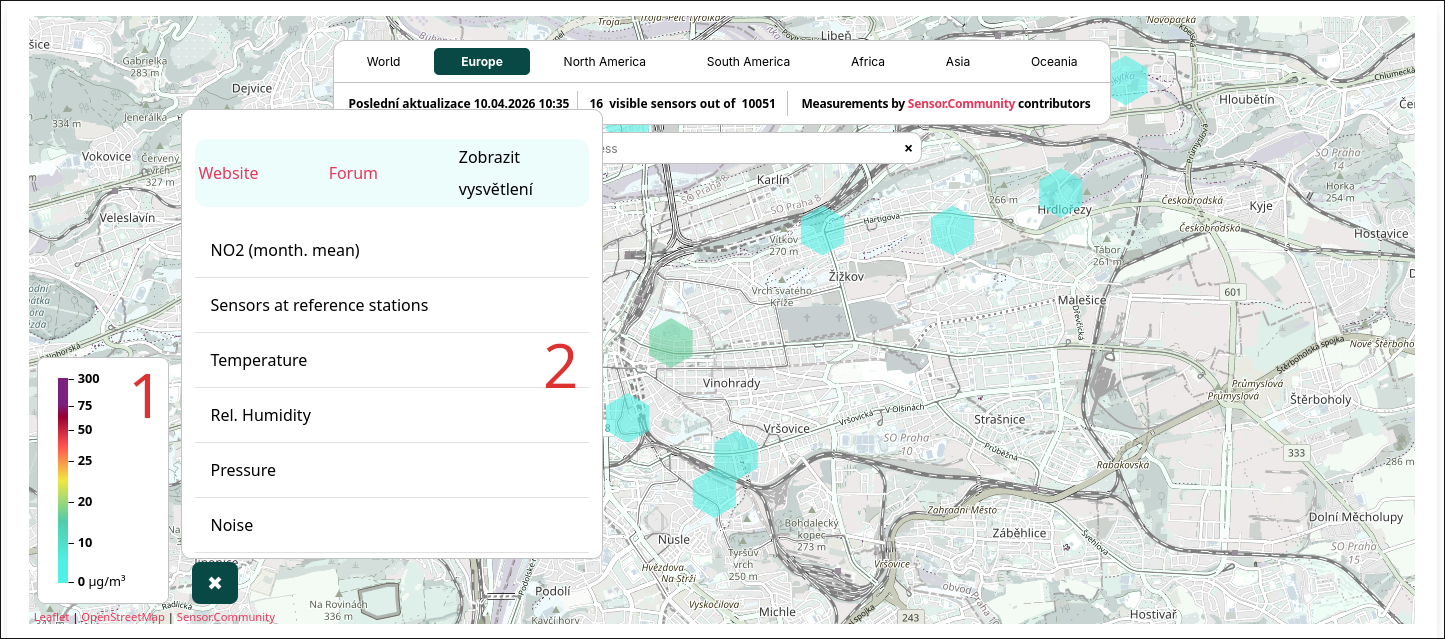
\includegraphics[width=.90\textwidth]{img/sensor-community-filtry}

\footnotesize \textit{Poznámka: 1 - barevná škála, 2 - filtry pro zobrazení dat na mapě.}

\footnotesize \textit{Zdroj:} Pořízeno autorem z webového rozhraní aplikace. 
\end{figure}

\begin{figure}[htbp!]\centering
\caption{Konkrétní senzor na mapě a jeho hodnota na webu \textit{sensor.community}}
\label{obr:sensor-community-sensor-reading}
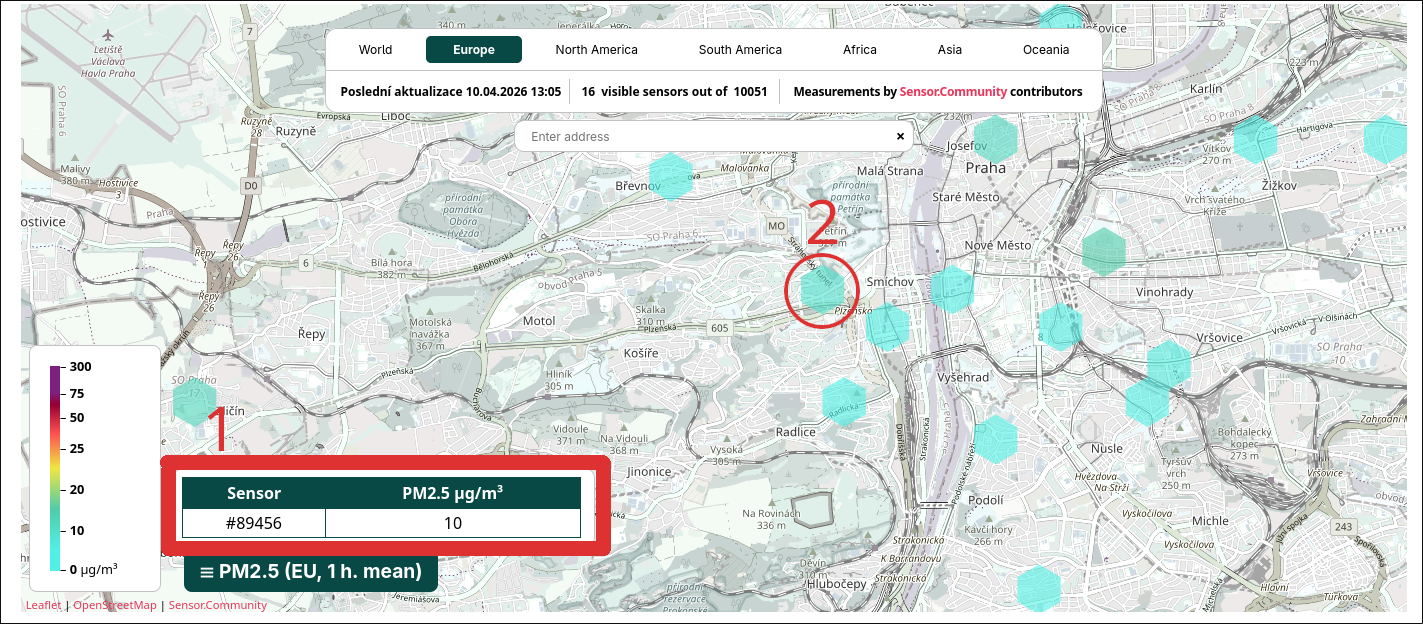
\includegraphics[width=.90\textwidth]{img/sensor-community-mapa-body}

\footnotesize \textit{Poznámka: 1 - konkrétní hodnota změřená vybraným senzorem, 2 - Klikatelný senzor na mapě. }

\footnotesize \textit{Zdroj:} Pořízeno autorem z webového rozhraní aplikace. 
\end{figure}

V tabulce č. \ref{tab:sensor-community-supported-sensors} je uveden přehled podporovaných senzorů aplikací Sensor.Community a veličin, které měří. V tabulce jsou uvedeny pouze veličiny, které jsou relevantní pro IEQ. Je nutné poznamenat, že aplikace v rámci některých senzorů nesbírá veškeré veličiny, které je daný senzor schopen měřit. Například u v rodině senzorů SEN5x existují senzory schopné měřit TVOC, ale v aplikaci, ať už v API, v CSV exportech nebo na webovém rozhraní, se veličina TVOC nevyskytuje. 

\clearpage
{
  \footnotesize
  \setlength{\tabcolsep}{2pt}
  \renewcommand{\arraystretch}{1.1}
  \begin{longtable}{*{1}{l}@{\hspace{12pt}}*{8}{c}@{\hspace{12pt}}*{3}{c}@{\hspace{12pt}}*{2}{c}@{\hspace{12pt}}*{2}{c}}
    \caption{Podporovné senzory sensor.community a jejich měřené veličiny}
    \label{tab:sensor-community-supported-sensors}\\
    \toprule
    \multirow{3}{*}{\textbf{Senzor}} & \multicolumn{15}{c}{\textbf{Kategorie IEQ}} \\
                                     & \multicolumn{8}{c}{\textbf{IAQ}} & \multicolumn{3}{c}{\textbf{TK}} & \multicolumn{2}{c}{\textbf{SK}} & \multicolumn{2}{c}{\textbf{AK}} \\
                                     & PM\textsubscript{2.5} & PM\textsubscript{10} & O\textsubscript{3} & NO\textsubscript{2} & SO\textsubscript{2} & CO & CO\textsubscript{2} & TVOC & $T$ & RH & $v$ & $E$ & CCT & $L_A$ & $L$ \\
                                     \hline
BME280 &  &  &  &  &  &  &  &  & \cmark & \cmark &  &  &  &  &  \\ % T, RH, P
\hline
BMP180 &  &  &  &  &  &  &  &  & \cmark &  &  &  &  &  &  \\ % T, P
\hline
BMP280 &  &  &  &  &  &  &  &  & \cmark &  &  &  &  &  &  \\ % T, P
\hline
DHT22 &  &  &  &  &  &  &  &  & \cmark & \cmark &  &  &  &  &  \\ % T, RH
\hline
DS18B20 & & & & & & & & & \cmark & & & & & &  \\ % T
\hline
DS18S20 & & & & & & & & & \cmark & & & & & & \\ % T
\hline
GPS-NEO-6M & & & & & & & & & & & & & & & \\ % GPS
\hline
HM3301 & \cmark & \cmark & & & & & & & & & & & & & \\ % PM1.0, PM2.5, PM10
\hline
HPM & \cmark & \cmark & & & & & & & & & & & & & \\ % PM2.5, PM10 output (standard); PM1.0, PM2.5, PM4.0
\hline
HTU21D & & & & & & & & & \cmark & \cmark & & & & & \\ % T, RH
\hline
IPS-7100 & \cmark & \cmark & & & & & & & & & & & & & \\ %PM (all)
\hline
DNMS (Laerm) & & & & & & & & & & & & & & \cmark & \\ % Noise
\hline
NextPM & \cmark & \cmark & & & & & & & & & & & & & \\ % PM2.5, PM10
\hline
NO2-A43F & & & & \cmark & & & & & & & & & & & \\ %NO2
\hline
PMS1003 & \cmark & & & & & & & & & & & & & & \\ %PM2.5, mozna PM10
\hline
PMS3003 & \cmark & & & & & & & & & & & & & & \\ %PM2.5
\hline
PMS5003 & \cmark & \cmark & & & & & & & & & & & & & \\ % PM1.0 PM2.5, PM10
\hline
PMS6003 & \cmark & & & & & & & & & & & & & & \\ %PM2.5
\hline
PMS7003 & \cmark & & & & & & & & & & & & & & \\ %PM2.5
\hline
PPD42NS & \cmark & & & & & & & & & & & & & & \\ %PM2.5, dust
\hline
Radiation SBM-19 & & & & & & & & & & & & & & & \\ %radiation
\hline
Radiation SBM-20 & & & & & & & & & & & & & & & \\ %radiation
\hline
Radiation Si22G & & & & & & & & & & & & & & & \\ %radiation
\hline
SCD30 & & & & & & & \cmark & & \cmark & \cmark & & & & & \\
\hline
SDS011 & \cmark & \cmark & & & & & & & & & & & & & \\
\hline
SDS021 & \cmark & \cmark & & & & & & & & & & & & & \\
\hline
SEN5x & \cmark & \cmark & & \cmark & & & & \cmark & \cmark & \cmark & & & & & \\
\hline
SHT10 & & & & & & & & & \cmark & \cmark & & & & & \\
\hline
SHT11 & & & & & & & & & \cmark & \cmark & & & & & \\
\hline
SHT15 & & & & & & & & & \cmark & \cmark & & & & & \\
\hline
SHT30 & & & & & & & & & \cmark & \cmark & & & & & \\
\hline
SHT31 & & & & & & & & & \cmark & \cmark & & & & & \\
\hline
SHT35 & & & & & & & & & \cmark & \cmark & & & & & \\
\hline
SHT85 & & & & & & & & & \cmark & \cmark & & & & & \\
\hline
SPS30 & \cmark & \cmark & & & & & & & & & & & & & \\
    \bottomrule
  \end{longtable}

  \footnotesize \textit{Zdroj: }Vlastní zpracování, \parencite{APISensorCommunity, SensorCommunityDevices}

  \footnotesize \textit{Poznámka:} Senzory \textit{Radiation SBM-19}, \textit{Radiation SBM-20} a \textit{Radiation Si22G} jsou určeny pro měření radiace, což autorem nebylo identifikováno jako měřená veličina relevantní pro IEQ. To samé se dá říci i o senzoru \textit{GPS-NEO-6M}, který je modulem GPS a má význam pouze pro lokalizaci senzoru.
}
\clearpage

